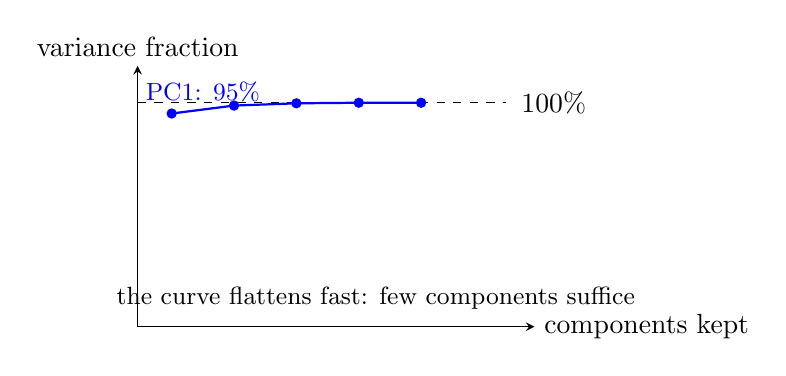
\begin{tikzpicture}[scale=0.72,>=stealth]
\draw[->] (0,0)--(7,0) node[right]{components kept};
\draw[->] (0,0)--(0,4.6) node[above]{variance fraction};
\draw[dashed] (0,3.95)--(6.5,3.95) node[right=2pt]{100\%};
% cumulative: 0.95, .987, .996, .999, 1.0
\draw[thick,blue,mark=*] plot coordinates {(0.6,3.76)(1.7,3.90)(2.8,3.94)(3.9,3.95)(5.0,3.95)};
\node[blue] at (1.15,4.15) {\small PC1: 95\%};
\node at (4.2,0.5) {\small the curve flattens fast: few components suffice};
\end{tikzpicture}
